\section{Inferential Statistics}
\subsection{Two-way analysis of variance(ANOVA)}
Our model is about using two-way ANOVA to determine the relationship between the dependent Processor Base Frequency with two independent which are number of Cores and Thermal Design Power(TDP). Because we want to check validity of this ANOVA model, we will have two assumption for this:\\
\\
\textbf{Normality}: Processor Base Frequency should be normal distribution for each combination of number of Cores and TDP.\\
\\
\textbf{Homogeneity}: Processor Base Frequency should be roughly across all combinations of number of Cores and TDP.
\subsubsection{Verify the assumption}
\textbf{Normality}: verify if the data is normal distribution\\
We use Shapiro-Wilk normality test to check if this model is normal distribution:\\
\\
\textbf{Null hypothesis $H_0$}: Processor Base Frequency should be approximately normally distributed for each combinations of number of Cores and TDP.\\
\\
\textbf{Alternative hypothesis $H_1$}: Processor Base Frequency should not be approximately normally distributed for each combinations of number of Cores and TDP.
\begin{figure}[H]
    \centering
    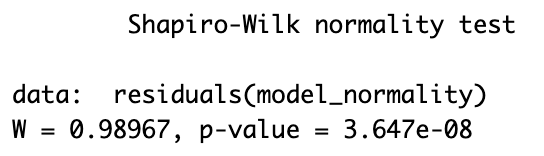
\includegraphics[width=0.8\textwidth]{graphics/shapiro.png}
    \caption{Shapiro-Wilk's test}
    \label{fig:shapiro}
\end{figure}
From the result, p-value is smaller than 0.05 so we reject $H_0$ and accept $H_1$. Therefore, Processor Base Frequency should not be approximately normally distributed for each combinations of number of Cores and TDP. So we need to plot out the model diagnose plot to check if it is normal distribution or not:
\begin{figure}[H]
    \centering
    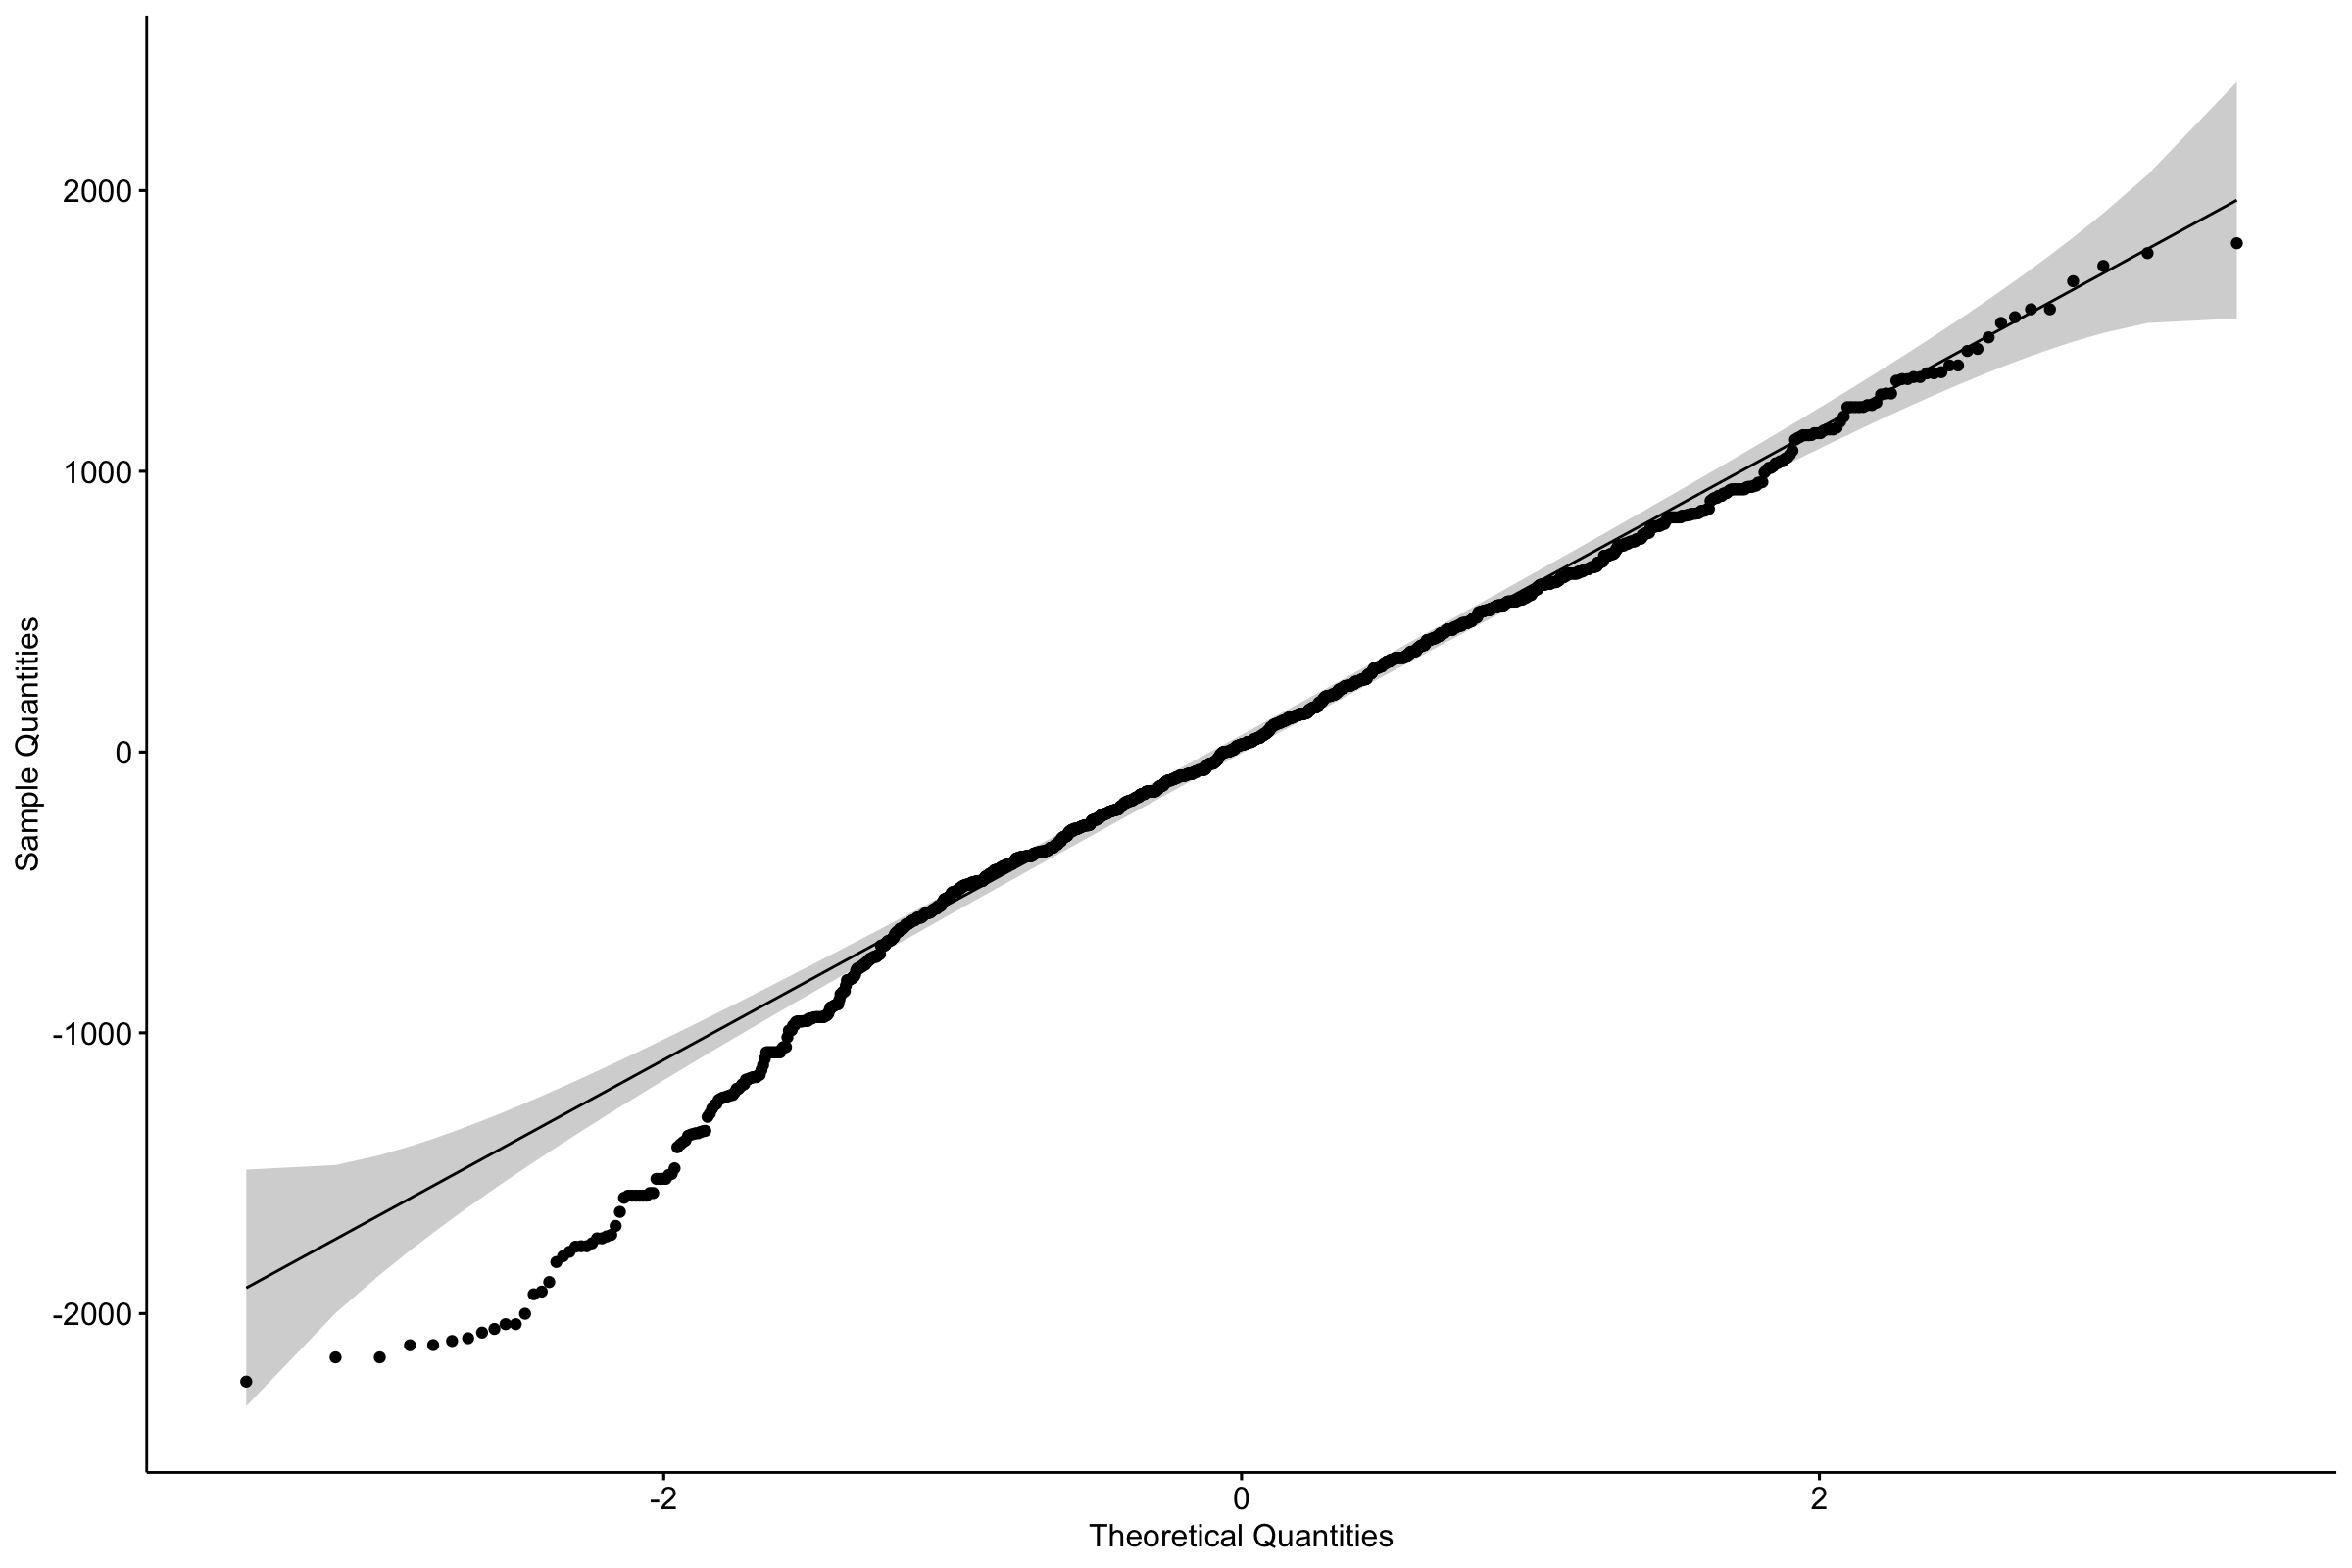
\includegraphics[width=1\textwidth]{graphics/check_normality.png}
    \caption{ggqqplot from ANOVA test}
    \label{fig:check_normality}
\end{figure}
We see that in ggqqplot, most of the points lie closely on the line. So we can assume that Processor Base Frequency is approximately normally distributed for each combinations of number of Cores and TDP.\\
\\
\textbf{Homogeneity}: verify the uniformity of the variance.\\
\\
We use Levene's test to check if this model is homogeneity:\\
\\
\textbf{Null hypothesis $H_0$}: Processor Base Frequency is homogeneity across groups of number of Cores and TDP.\\
\\
\textbf{Alternative hypothesis $H_1$}: Processor Base Frequency is not homogeneity across groups of number of Cores and TDP.
\begin{figure}[H]
    \centering
    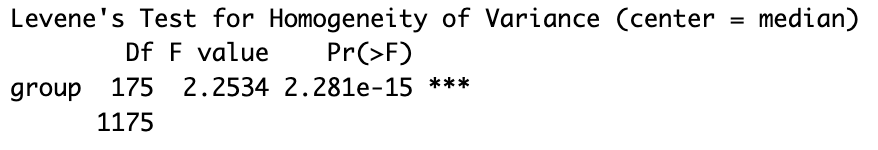
\includegraphics[width=1\textwidth]{graphics/check_homogeneity.png}
    \caption{Leneve's Test for Homogeneity of Variance}
    \label{fig:check_homogeneity}
\end{figure}
From the result, we see that p-value is smaller than 0.05 so we reject $H_0$ and accept $H_1$. Therefore, Processor Base Frequency is not homogeneity across groups of number of Cores and TDP. 
\subsubsection{Calculate ANOVA}
\textbf{Null hypothesis $H_0$}: Processor Base Frequency follows the same distribution across group defined by the independent variables number of Cores and TDP.\\
\\
\textbf{Alternative hypothesis $H_1$}: Processor Base Frequency follows different distribution across group defined by the independent variables number of Cores and TDP.
\begin{figure}[H]
    \centering
    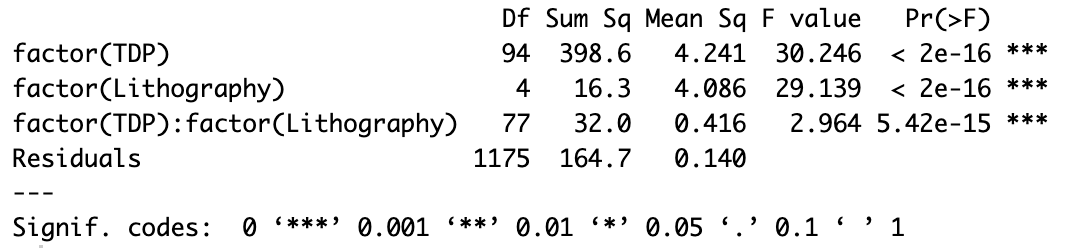
\includegraphics[width=1\textwidth]{graphics/anova_test.png}
    \caption{Calculate ANOVA}
    \label{fig:calculate_anova}
\end{figure}
From the result, we see that Pr(>F) value is smaller than 0.05 so we reject $H_0$ and accept $H_1$. Therefore, Processor Base Frequency follows different distribution across group defined by the independent variables number of Cores and TDP.

\subsection{Multiple Linear Regression to Predict CPU Clock Speed}

\subsubsection{Data Splitting}
After finalizing the data we need for statistical analysis, we have to split the data further into two subsets: \textbf{training set and test set}. Training set helps us build and train the model, allowing it to learn the patterns and connections within our data. Then, the test set will be tested on the validated model to give an objective assessment of the model's efficacy and performance on fresh, unseen data. In data science and machine learning, this train-test split strategy is a standard procedure since it ensures that the model generalises effectively to new data and helps prevent over-fitting. In this project, the training set consists of 70\% of the original data, and the remaining 30\% makes up the test set.

%%%%%% Khúc này là code format lại giùm nha %%%%%%
smp_size <- floor(0.70 * nrow(intel_cpu_subset))
set.seed(123)
train_ind <- sample(seq_len(nrow(intel_cpu_subset)), size = smp_size)

train_set <- intel_cpu_subset[train_ind, ]
test_set <- intel_cpu_subset[-train_ind, ]
%%%%%%%%%%%%%%%%%%%%%%%%%%%%%%%%%%%%%%%%%%%%%%%%%%
%% Chú thích ở dưới: Code served for data splitting

\subsubsection{Regression Model}
The main objective of this section is constructing a model that portrays the effect of other factors on the CPU clock speed. To achieve this we applied a Multi Regression model, in which the dependent variable is Processor Base Frequency - the variable representing CPU clock speed, and the rest are independent. Our model appears as the formula below:\\

$Processor Base Frequency = \beta_0 + \beta_1 nb\_of\_Cores + \beta_2 nb\_of\_Threads + \beta_3 TDP + \beta_4 Lithography$ \\

We start with our \textbf{first model}, also known as the \textbf{base model}, built with all the independent variables available. \\

%%%%%% Khúc này là kqua format lại giùm nha %%%%%%
Call:
lm(formula = Processor_Base_Frequency ~ nb_of_Cores + nb_of_Threads + 
    TDP + Lithography, data = train_set)

Residuals:
     Min       1Q   Median       3Q      Max 
-1.63836 -0.27698  0.01221  0.31291  1.17039 

Coefficients:
               Estimate Std. Error t value Pr(>|t|)    
(Intercept)    2.813706   0.050545  55.668  < 2e-16 ***
nb_of_Cores   -0.127859   0.017229  -7.421 2.59e-13 ***
nb_of_Threads  0.000201   0.008336   0.024    0.981    
TDP            0.016153   0.000503  32.113  < 2e-16 ***
Lithography   -0.032354   0.001757 -18.416  < 2e-16 ***
---
Signif. codes:  0 ‘***’ 0.001 ‘**’ 0.01 ‘*’ 0.05 ‘.’ 0.1 ‘ ’ 1

Residual standard error: 0.4579 on 940 degrees of freedom
Multiple R-squared:  0.5423,	Adjusted R-squared:  0.5404 
F-statistic: 278.5 on 4 and 940 DF,  p-value: < 2.2e-16
%%%%%%%%%%%%%%%%%%%%%%%%%%%%%%%%%%%%%%%%%%%%%%%%%%


In this model, our respone variables consist of: nb\_of\_Cores, nb\_of\_Threads, TDP and Lithography. Now, we should remove the variables that are proven insignificant to our analysis, which can be determined based on their Pr values (last column). If $Pr < 0.05$, the variable is significant. With this insight, the variable that will be deducted is nb\_of\_Threads. Subsequently, we now construct the \textbf{new and theoretically improved model}. \\

%%%%%% Khúc này là kqua format lại giùm nha %%%%%%
Call:
lm(formula = Processor_Base_Frequency ~ nb_of_Cores + TDP + Lithography, 
    data = train_set)

Residuals:
     Min       1Q   Median       3Q      Max 
-1.63831 -0.27754  0.01245  0.31306  1.17061 

Coefficients:
              Estimate Std. Error t value Pr(>|t|)    
(Intercept)  2.8133773  0.0486411   57.84   <2e-16 ***
nb_of_Cores -0.1274613  0.0050185  -25.40   <2e-16 ***
TDP          0.0161541  0.0004978   32.45   <2e-16 ***
Lithography -0.0323520  0.0017534  -18.45   <2e-16 ***
---
Signif. codes:  0 ‘***’ 0.001 ‘**’ 0.01 ‘*’ 0.05 ‘.’ 0.1 ‘ ’ 1

Residual standard error: 0.4577 on 941 degrees of freedom
Multiple R-squared:  0.5423,	Adjusted R-squared:  0.5409 
F-statistic: 371.7 on 3 and 941 DF,  p-value: < 2.2e-16
%%%%%%%%%%%%%%%%%%%%%%%%%%%%%%%%%%%%%%%%%%%%%%%%%%

However, our group came to the decision of using the base model, since the difference in Adjusted $R^2$ value between the two is not significant enough (0.0001) to implement the second model as an improvement over the first. Hence, our final model now should look like this:\\

$Processor Base Frequency = 2.8134 - 0.1279 \cdot nb\_of\_Cores + 0.0002 \cdot nb\_of\_Threads + 0.0162 \cdot TDP - 0.0324 \cdot Lithography$ \\

Observing the results R gave on model 2, the p - value correlating with F statistics is less than $2.2 \cdot 10^{-16}$. This suggests that our data is robust and valuable for statistical analysis. Additionally, it guarantees that future results from this model provide good evaluations about the relationship between the Processor Base Frequency and the remaining variables. Generally, the regression coefficients ($\beta_i$) and the p - values hold the most influences on the independent variables. 

\subsubsection{Assumptions of Linear Regression}

% ảnh giả định

\subsubsection{Testing}
We first run the model on our \textbf{training set} (70\% of the original data) to validate the model before actual testing. To gauge the correspondence between our estimates and the actual values, we look at their distribution and compare them.\\

%graph train set

The values plotted on this graph is quite widely distributed from the regression line, proving that the predicted and actual values form an average linear relationship. This confirms that the model is effective.\\

We now run the model on the preceding \textbf{test set} (30\% of the original data) to access the performance of our model. Then, we put the predicted values into a new column in the dataset for easy plotting.\\

%%%%%% Khúc này là code format lại giùm nha %%%%%%
predicted\_values <- predict(regression\_model, test\_set)
test\_set["Predicted"] <- predicted\_values
%%%%%%%%%%%%%%%%%%%%%%%%%%%%%%%%%%%%%%%%%%%%%%%%%%

Then we plot the graph following the exact same way as we did with the training set.\\

%graph test set

The graph portrays a linear relationship between the predicted and actual values, indicating that the model works on unseen data. This concludes that this model is good at predicting the clock speed based on the key variables mentioned.

\subsection{Conclusion}
After implementing a Multi Regression Model to predict the CPU Clock Speed, we were able to identified 4 variables that are significant to the Processor Base Frequency. The model aid manufacturers in pinpointing the factors that affect the CPU performance through its clock speed, providing appropriate strategies in product development, while also help customer choosing the right CPU specifications for their needs. Overall, the results that the model predict is justifiably similar to the actual data. 
\newpage
